\subsubsection{Introduction}\label{mqintro}

Due to the limitations in the previous experiment, a new system was introduced, built around a central message queue.

\subsection{Message Queues}
\hypertarget{introduction}{%
\subsubsection{Introduction}\label{introduction}}

A problem exists in the architecture described in the prior section.
At base, the co-ordination between nodes in the
cluster requires significant effort from the master, with little room
for additional features, with all inter-node communication being remote
procedure calls only. This issue compromises nearly every aspect of
operations on distributed objects, particularly in the initial reading
in of data, and later data movement. The proposed amendments as
described in \href{current-proposed-info-structures.html}{Proposed
Information Structures} provide some degree of amelioration, however the
root of the issue in requiring full co-ordinating facilities from the
master node is still not solved.

A potential solution exists in the use of message queues. Message queues
are commonly used for inter-process communication, consisting of queues
through which applications may communicate over \cite{curry2004message}.
The use of message queues for communication between nodes will allow for
significantly less knowledge required about other nodes within the
system, and enabling greater independence of action within each node.
Further benefits include allowing for asynchrony in more operations, the
ability to monitor the system externally through watching queues, as
well as the attendant benefits of decentralisation such as potentially
greater resilience and decreased central complexity.

Message queues are well established, seeing use from Operating Systems
to Web Services. For example, the QNX OS makes heavy use of message
queues for its microkernel architecture \cite{hildebrand1992qnx}. Tech
companies Stack Overflow and flickr also use message queues from redis
as central components of their infrastructure \cite{nolan2011flickr}
\cite{montrose2016stack}. In this platform, the flexibility of Redis lists
and the availability of the rediscc package suggests the use of Redis in
the implementation of message queues \cite{sanfilippo2009redis}
\cite{urbanek2020rediscc}. Alternatives include Apache ActiveMQ, Kafka, and
Disque, among others \cite{snyder2011activemq}\cite{garg2013kafka}
\cite{sanfilippo2016disque}.

\hypertarget{architecture-concept}{%
\subsubsection{Architecture Concept}\label{architecture-concept}}

The concept retains the notion of data divided into uniquely identified
chunks, existing on nodes. The nodes each subscribe to queues dedicated
to chunks that they possess, undertaking action dependent on messages
received in their queue. In this way, nodes function as state machines,
reading messages, performing some operation (or not) depending on the
message content, and writing back in some form.

For example, some node has a chunk \(x\), and receives a message on the
\(x\) queue to add it to another chunk \(y\); if it didn't have the
chunk \(y\), it may post a message on the \(y\) queue, requesting it. It
is likely that the semantics are more general, and the initial message
of operation actually won't specify which chunk to add to \(x\), giving
it a more general request of addition between distributed objects, and
the node will have to determine for itself which chunks to pull to it,
if any.

A very simple example is given by \cref{lst:msg-q-master}
\cref{lst:msg-q-worker}, demonstrating the master and worker node routines
respectively.

\hypertarget{lst:msg-q-master}{%
\label{lst:msg-q-master}}%
\begin{verbatim}
library(rediscc)

REDIS_HOST <- "localhost"
REDIS_PORT <- 6379L
QUEUE <- "chunk"
MSG <- quote({ chunk + 1})

main <- function() {
    rsc <- redis.connect(REDIS_HOST, REDIS_PORT)
    writeMsg(MSG, to=QUEUE, conn=rsc)
}

writeMsg <- function(msg, to, conn) {
    serializedMsg <- rawToChar(serialize(msg, NULL, T))
    redis.push(conn, to, serializedMsg)
}

main()
\end{verbatim}

\hypertarget{lst:msg-q-worker}{%
\label{lst:msg-q-worker}}%
\begin{verbatim}
library(rediscc)

REDIS_HOST <- "LOCALHOST"
REDIS_PORT <- 6379L
QUEUE <- "chunk"
chunk <- seq(10)

main <- function() {
    rsc <- redis.connect(REDIS_HOST, REDIS_PORT)
    while (TRUE) {
        msg <- readMessage(QUEUE, conn=rsc)
        print(eval(msg))
    }
}

readMessage <- function(queues, conn) {
    serializedMsg <- redis.pop(conn, queues, timeout=Inf)
    unserialize(charToRaw(serializedMsg))
}

main()
\end{verbatim}

The master simply pushes serialised calls to the appropriate queue, and
the worker loops reading messages from it's particular queue(s),
unserialising and evaluating any messages. The master node and the
worker node can be initialised in any order and with any time
difference, demonstrating the asynchrony. In this particular example,
the master puts out a call to add the number 1 to a predefined chunk
named ``chunk'', with the worker executing the call as expected. The
master doesn't have to have any knowledge about where the chunk exists,
and the worker likewise doesn't necessarily require information on where
the message originated from.

With relation to the queues, the aggregate functionality of nodes in a
cluster, can be considered distinctly to the functionality of a singular
node. The cluster must have some means of initialising the queues to
listen to for the individual nodes, for the reading in of an external
dataset. The process of operating based on queues is straightforward at
the outset, but requires considerable thought on the representation and
existence of objects other than the referent object of a queue when the
queues operations require those other objects.

The issue of data movement also requires consideration; while this is
largely an implementation-specific issue, it has a strong bearing on
conceptual architecture. These three considerations mirror the state
machine concept at an aggregate level, with resultant decisions
affecting the architecture at large.

\hypertarget{plausible-extensions}{%
\subsubsection{Plausible Extensions}\label{plausible-extensions}}

While the use of message queues looks to ease many significant issues,
there are additional problems that it require addressing, primarily
resulting from the asynchrony and decentralisation.

Most pressingly, the issue of deadlock, in the context of data movement
in the process of nodes requesting and transferring data, a deadlock is
almost certain to occur if not dealt with. This specific instance may be
helped through careful implementation and more processing on the
initiator node (bringing it closer to a master node), but a possibly
superior extension is to have queue-adjacent servers on each node that
are able to operate concurrently with the main \R session that has as
it's sole purpose the transfer of chunks, leaving everything else to the
main \R session. These servers would also be ideal vertices at which to
implement data-duplication as a feature enabling redundancy in the
system

In a similar vein, failure detection can be implemented through a
concurrent ``heartbeat'' server, in the same manner as \pkg{Hadoop}
\cite{white20122adoop}.

These extensions are worth bearing in mind for now, however the
considerations brought up in the prior section need to be answered
first.

\subsection{Chunks in the Central Message Queue}

\subsubsection{Introduction}

Given the simplicity and promise of flexibility as demonstrated in the
documents \href{inter-node-comm-w-redis.pdf}{Inter-node Communication with
Redis} and \href{message-queues-comms.pdf}{Message Queue Communications},
further experimentation around the concept is undertaken and documented herein.
The experiments are built successively upon it's prior, with the aim of rapidly
approximating a functioning prototype via experimentation.

\subsubsection{General Function on Single Chunk}

While the RPC-based architecture as described in
\href{experiment-eager-dist-obj-pre.pdf}{Experiment: Eager Distributed Object}
had significant limitations, a particularly powerful construct was the higher
order function \mintinline{r}{distributed.do.call}, which took functions as arguments
to be performed on the distributed chunks.

This construct is powerful in that it can serve as the basis for nearly every
function on distributed chunks, and this section serves to document experiments
relating to the creation of a general function that will perform a function at
the node hosting a particular chunk.

\subsubsection{With Value Return}\label{sec:val-ret}

Regardless of performing the actual function, some means of returning the value
of a function must be provided; this section focuses on getting a function to
be performed on a server node, with the result send back to the client.
Listings of an implementation of these concepts are given by listings
\cref{src:vr-client} and \cref{src:vr-server}.

To this end, the client node has a function defined as \texttt{doFunAt(fun,
chunk)}, which takes in any function, and the ID of a chunk to perform the
function on.
An implementation is given by listing \cref{src:vr-client}.
\texttt{doFunAt} first composes a message to send to the chunk's queue, being a
list consisting of the function, the chunk name, and a return address, which
contains sufficient information for the node performing the operation on the
chunk to send the results back to via socket connection.
The message is then serialised and pushed to the chunk's queue, and the
requesting node sits listening on the socket that it has set up and advertised.

On the server node end, it sits waiting on it's preassigned queues, each of
which correspond to a chunk that it holds. 
Upon a message coming through, it runs a \texttt{doFun} function on the
message, which in turn runs the function on the chunk named in the message. 
An implementation is given by listing \cref{src:vr-server}.
It then creates a socket connected to the clients location as advertised in
the message, and sends the serialised results through.

A problem with this approach is the fickle aspect of creating and removing
sockets for every request; beyond the probability of missed connections and
high downtime due to client waiting on a response, \R only has a very limited
number of connections available to it, so it is impossible to scale beyond that
limit.

\subsubsection{With Assignment}

Assigning the results of distributed operation to a new chunk is a far more
common operation in a distributed system in order to minimise data movement.
This will involve specifying additional directions as part of the request
message, in order to specify that assignment, and not merely the operation, is
desired.

It will be clear from the previous example that the problem of point-to-point
data movement, somewhat solved via direct sockets in that previous example, is
largely an implementation issue, and a problem entirely distinct to the
remainder of the logic of the system.
From this experiment onwards, the mechanism of data movement is abstracted out,
with the assumption that there will exist some additional tool that can serve
as a sufficient backend for data movement.
In reality, until that tool is developed, data will be sent through redis; not
a solution, but something that can be ignored without loss of generality.

The actual creation of a chunk ID in itself demands a system-wide unique
identifier; this is a solved problem with a central message server, in redis
providing an \texttt{INCR} operation, which can be used to generate a new chunk
ID that is globally unique.

The name origination and option of blocking until a chunk is formed will
dictate different algorithms in the creation of the distributed chunk object,
as well as the structure of the distributed chunk object.
Table \cref{tab:name-orig-block} shows potential forms these may take.
In addition, the ``job ID'' referred to in the table may
take the concrete form of a simple key-value store, with the key being passed
and monitored by the client node.

\begin{table}
	\centering
	\caption{Description of Algorithms and Data Structure of chunk
	reference object, by blocking status in creation, and origination of
	chunk ID.}
	\label{tab:name-orig-block}
	\begin{tabularx}{\textwidth}{l|XX}
	\toprule
	& Client-Originated chunk ID & Server-Originated chunk ID \\
	\midrule
	Blocking Algorithm & 
		client attains chunk ID, sends operation request with
		chunk ID to server, creating chunk reference concurrently,
		blocking until direct signal of completion from server. & 
		client sends operation request with reference to some common
		information repository and the job ID to server. server attains
		chunk ID, performs operation, and sends chunk chunk ID to the
		job ID at the common information repository, which client
		watches, releasing chunk object after attaining chunk ID from
		repository. \\
	Blocking Structure & 
		String name of chunk. & 
		String name of chunk. \\
	Non-Blocking Algorithm & 
		client attains chunk ID, sends operation request with
		chunk ID to server, creating chunk reference concurrently. No
		waiting for server signal of completion. & 
		client sends operation request with reference to some common
		information repository and the job ID to server. server attains chunk ID, performs
		operation, and sends chunk ID to the job ID at common information
		repository. Before server completion, client releases chunk
		object, not waiting for reception of chunk information. \\
	Non-Blocking Structure & 
		String name of chunk &
		Initially, reference to common information repository. Mutable;
		can become string name of chunk upon accessing that information
		in the common information repository. \\
	\bottomrule
\end{tabularx}
\end{table}

While it is clearly more straightforward for a client node to originate a chunk
ID, with blocking, the opposite will possibly be the most flexible;
server-originated chunk ID with no blocking.
This is because the very existence of a chunk is presupposed when a client
node originates a chunk ID, while that may not be true in reality.
For instance, the result may be an unexpected \texttt{NULL}, zero-length
vector, or even an error.
In addition, the server-originated chunk ID with no blocking has every feature
common to that of a future, from the future package; it can be checked for
completion, and accessed as a value, allowing for many asynchronous and
parallel operations.

\subsubsection{Client-Originated Chunk ID}

The logic of the client in assigning the result of a distributed operation on a
chunk is largely encapsulated in a new function, \texttt{assignFunAt}, as
demonstrated in listing \cref{src:ro-ass-client}.
The function attains a chunk ID, generates a unique return address, sends a
message to the operand chunk queue, and waits for a reply, before returning the
id as a string belonging to the ``chunk'' class.
There is more information in the message relative the the function-only
message of section \cref{sec:val-ret}; the chunk ID, request for acknowledgement
of completion, return address, as well as an operation specifier to direct the
intent of the message.

The server, as shown in listing \cref{src:ro-ass-server}, consists in a loop of
reading the message and performing an operation dependent on the operation
specifier of the message.
For an operation of \texttt{DOFUN}, all that is run is a \texttt{do.call} on
the function and chunk specified, with a message being returned to the
client with the value of the \texttt{do.call}.
An operation of \texttt{ASSIGN} runs the same as \texttt{DOFUN}, with the
addition of assigning the value to the ID as passed in the message, adding
the ID to the array of queues to monitor, and potentially sending
acknowledgement back to the client node.

\subsubsection{Server-Originated chunk ID}

By this point the client (listing \cref{src:wo-ass-client}) and server (listing
\cref{src:wo-ass-server}) come to increasingly resemble each other, and most of
the functions are shared, as in listings \cref{src:wo-ass-chunk},
\cref{src:wo-ass-shared}, and \cref{src:wo-ass-messages}.

The principal mechanism of action is best demonstrated via a logical time
diagram, given by figure \cref{fig:w-o-td}, following a Lamport form of
event ordering\cite{lamport1978ordering}.
The first message, shown by the \textbf{a} arrow in the diagram, involves a
client sending a message to a server regarding the request, including the job
ID naming a queue in a shared information reference for the server to later
place the chunk ID into.

Optionally, the client can immediately create a chunk object with no direct
knowledge of the chunk ID, holding the job ID at the information reference
instead, and the client continues whatever work it was doing.
Only when the chunk ID is required, the chunk object, triggers a blocking pop
on it's associated information reference queue, which the server may
at any point push the chunk ID to.
The chunk object then has the associate the ID associated with it, and the
information reference queue can be deleted.

\begin{figure}
	\begin{minipage}{0.4\textwidth}
	\begin{tikzpicture}
		\draw[-{>[scale=2]}] (0,8) -- (0,0) node[at start, anchor=south] {C};
		\draw[-{>[scale=2]}] (2,8) -- (2,0) node[at start, anchor=south] {Q};
		\draw[-{>[scale=2]}] (4,8) -- (4,0) node[at start, anchor=south] {S};

		\draw[red] (0,7.5) -- (0,3) node[midway, anchor=east] {x};
		\draw[red] (4,5) -- (4,4.5) node[midway, anchor=west] {y};

		\draw[-{>[scale=2]}] (0,7.5) -- (2, 6.5) node[midway, anchor=south] {a};
		\draw[-{>[scale=2]}] (4,8) -- (2, 7) node[midway, anchor=south] {b};
		\draw[-{>[scale=2]}] (2, 6) -- (4, 5) node[midway, anchor=south] {c};
		\draw[-{>[scale=2]}] (4, 4.5) -- (2, 3.5) node[midway, anchor=south] {d};
		\draw[-{>[scale=2]}] (0, 3) -- (2, 2) node[midway, anchor=south] {e};
		\draw[-{>[scale=2]}] (2, 1.5) -- (0, 0.5) node[midway, anchor=south] {f};
	\end{tikzpicture}
\end{minipage}\begin{minipage}{0.6\textwidth}
	\begin{description}
		\item [a] Assignment request message pushed to chunk
			queue
		\item [b] Blocking pop of queue
		\item [c] Message popped from queue
		\item [d] Chunk ID pushed to information reference
			queue
		\item [e] Request for chunk ID creates blocking pop for
			information reference queue
		\item [f] Chunk ID message popped from information
			reference queue
		\item [\textcolor{red}{x}] Creation of chunk object
			containing job ID, but no chunk ID, followed by
			any operations not requiring chunk ID
		\item [\textcolor{red}{y}] Perform operation specified
			by message in \textbf{e}, with assignment
	\end{description}
\end{minipage}

	\caption{\label{fig:w-o-td}Logical time diagram of chunk assignment for
	server-originated chunk ID}
\end{figure}

\subsection{Chunk Identification}

\subsubsection{Introduction}

The problem of chunk ID origination as discussed in
\href{init-chunk-msg-q-exp.pdf}{Initial Chunk Message Queue Experiments}
dictates much of the client-server communication, as well as the state of
knowledge in the network, given that chunk ID is used as the key to send
messages relevant to a particular chunk.
This document serves to model the differences between naive client-originated
chunk ID's, and server-originated chunk ID's, with an evaluation and proposal
that aims at overcoming the limitations involved in the models.

\subsubsection{Modelling}\label{sec:cid-model}

The models consist of communication over time between a client and a server,
intermediated by a queue server.
The client runs the pseudo-program described in listing \cref{src:client-p},
where variables \texttt{x}, \texttt{y}, and \texttt{z} are chunk references,
and variables \texttt{i} and \texttt{j} are local. 
Every action on distributed chunk references entails pushing a  message to the
queue named by the associated chunk ID, requesting the relevant action to be
performed.

\begin{listing}
\begin{minted}{r}
	y <- f(x)	# dist, no wait
	f(i)		# local
	z <- f(y)	# dist, no wait
	f(j)		# local
	f(z)		# dist, wait
\end{minted}
\caption{Modelled Client Program}\label{src:client-p}
\end{listing}

The server follows a loop of listening on queues relevant to the chunks that it
stores and performing requests from the messages popped in order from them,
through taking the function relayed in the message and performing it on the
local object identified by the chunk ID given by the queue name the message was
popped from.
Without loss of generality, the function \texttt{f} is considered to take
constant time on local objects, and messages likewise have constant latency;
the ratio of latency to operation time is irrelevent to what is demonstrated in
these models.
Assignment, message listening, and message switching by the queue are
considered to be instantaneous events.
The models are depicted as space-time diagrams, with modifications to the
original styling\cite{lamport1978ordering}, including colour coding, where the
colours aim to make each job more distinct.

\subsubsection{Client-Originated Chunk ID}

In the client-originated chunk ID  model, in addition to the generic model
description posed in section \cref{sec:cid-model}, the client sends a chunk ID
as part of its messages if the result of the function on the distributed object
includes assignment.
If there is no assignment, the message includes a job ID instead, naming a job
queue to be monitored by the client.
If the server receives a job ID, it sends the value of the computed function to
the queue with that job ID as it's key, sending no messages otherwise.

A space-time diagram of the client-originated chunk ID model is given in figure
\cref{fig:mci}.

\begin{figure}
		\begin{minipage}{0.6\textwidth}
	\begin{tikzpicture}
		% nodes
		\draw[very thin,-{>[scale=2]}] (0,10) -- (0,0) 
			node[at start,anchor=south] {C};
		\draw[very thin,-{>[scale=2]}] (2,10) -- (2,0) 
			node[at start,anchor=south] {Q};
		\draw[very thin,-{>[scale=2]}] (4,10) -- (4,0) 
			node[at start,anchor=south] {S};

		% listeners
		\draw[color=mygray] (4,9.5) -- (2,9.5) 
			node[midway,anchor=south] {b};
		\draw[color=dark2-5] (0,7.5) -- (2,7.5) 
			node[midway,anchor=south] {e};
		\draw[color=mygray] (4,7.5) -- (2,7.5) 
			node[midway,anchor=south] {g};
		\draw[color=mygray] (4,6) -- (2,6) 
			node[midway,anchor=south] {i};
		\draw[color=mygray] (4,4.5) -- (2,4.5) 
			node[midway,anchor=south] {k};

		% y <- f(x)
		\draw[-{>[scale=2]},dark2-1] (0,9.5) -- (2,9) 
			node[at start,anchor=east] {\texttt{y <- f(x)}}
			node[midway,anchor=south] {a};
		\draw[-{>[scale=2]},dark2-1] (2,9) -- (4,8.5)
			node[midway,anchor=south] {c};
		\draw[very thick,dark2-1] (4,8.5) -- (4,7.5) 
			node[midway,anchor=west] {\texttt{C2 <- f(C1)}};

		% f(i)
		\draw[very thick,dark2-2] (0,9.5) -- (0,8.5) 
			node[midway,anchor=east] {\texttt{f(i)}};

		% z <- f(y)
		\draw[-{>[scale=2]},dark2-3] (0,8.5) -- (2,8) 
			node[at start,anchor=east] {\texttt{z <- f(y)}}
			node[midway,anchor=south] {d};
		\draw[-{>[scale=2]},dark2-3] (2,7.5) -- (4,7)
			node[midway,anchor=north] {h};
		\draw[very thick,dark2-3] (4,7) -- (4,6) 
			node[midway,anchor=west] {\texttt{f(C2)}};

		% f(j)
		\draw[very thick,dark2-4] (0,8.5) -- (0,7.5)
			node[midway,anchor=east] {\texttt{f(j)}};
			
		% f(z)
		\draw[-{>[scale=2]},dark2-5] (0,7.5) -- (2,7) 
			node[at start,anchor=east] {\texttt{f(z)}}
			node[midway,anchor=north] {f};
		\draw[-{>[scale=2]},dark2-5] (2,6) -- (4,5.5)
			node[midway,anchor=north] {j};
		\draw[very thick,dark2-5] (4,5.5) -- (4,4.5) 
			node[midway,anchor=west] {\texttt{f(C3)}};
		\draw[-{>[scale=2]},dark2-5] (4,4.5) -- (2,4)
			node[midway,anchor=north] {l};
		\draw[-{>[scale=2]},dark2-5] (2,4) -- (0,3.5)
			node[midway,anchor=south] {m};
	\end{tikzpicture}
	\end{minipage}
	\begin{minipage}{0.4\textwidth}
		\begin{description}
			\item [\textcolor{dark2-1}{a}] Push \texttt{<f, chunkID=C2>} to queue \texttt{C1}
			\item [\textcolor{mygray}{b}] Listen to queue \texttt{C1}
			\item [\textcolor{dark2-1}{c}] Pop \texttt{<f, chunkID=C2>} from queue \texttt{C1}
			\item [\textcolor{dark2-3}{d}] Push \texttt{<f, chunkID=C3>} to queue \texttt{C2}
			\item [\textcolor{dark2-5}{e}] Listen to queue \texttt{C3}
			\item [\textcolor{dark2-5}{f}] Push \texttt{<f, jobID=J1>} to queue \texttt{C3}
			\item [\textcolor{mygray}{g}] Listen to queues \texttt{C1, C2}
			\item [\textcolor{dark2-3}{h}] Pop \texttt{<f, chunkID=C3>} from queue \texttt{C2}
			\item [\textcolor{mygray}{i}] Listen to queues \texttt{C1, C2, C3}
			\item [\textcolor{dark2-5}{j}] Pop \texttt{<f, jobID=J1>} from queue \texttt{C3}
			\item [\textcolor{mygray}{k}] Listen to queues \texttt{C1, C2, C3}
			\item [\textcolor{dark2-5}{l}] Push \texttt{<val>} to queue \texttt{J1}
			\item [\textcolor{dark2-5}{m}] Pop \texttt{<val>} from queue \texttt{J1}
		\end{description}
	\end{minipage}

	\caption{\label{fig:mci} Space-Time Diagram of Client-Originated Chunk ID}
\end{figure}

\subsubsection{Server-Originated Chunk ID}

In the server-originated chunk ID model, given that the client doesn't know the
chunk ID of created chunk references, leaving that to the server, it sends out
messages with job IDs, creating chunks references that at first reference the
job ID, but when the actual chunk ID is required, waiting on the job ID queue
for a message containing it's chunk ID.
The server correspondingly sends chunk IDs of each newly assigned chunk to the
job ID queue specified in the request, sending values instead if not directed
to perform assignment.

A diagram of the server-originated chunk ID model is given in figure \cref{fig:msi}.

\setlength{\columnsep}{50pt}
\begin{figure}
	\centering
		\begin{tikzpicture}
		% nodes
		\draw[very thin,-{>[scale=2]}] (0,10) -- (0,0) 
			node[at start,anchor=south] {C};
		\draw[very thin,-{>[scale=2]}] (2,10) -- (2,0) 
			node[at start,anchor=south] {Q};
		\draw[very thin,-{>[scale=2]}] (4,10) -- (4,0) 
			node[at start,anchor=south] {S};

		% listeners
		\draw[color=mygray] (4,9.5) -- (2,9.5) 
			node[midway,anchor=south] {b};
		\draw[color=dark2-3] (0,8.5) -- (2,8.5) 
			node[midway,anchor=south] {d};
		\draw[color=mygray] (4,7.5) -- (2,7.5) 
			node[midway,anchor=south] {e};
		\draw[color=dark2-5] (0,5.5) -- (2,5.5) 
			node[midway,anchor=south] {j};
		\draw[color=mygray] (4,4.5) -- (2,4.5) 
			node[midway,anchor=south] {k};
		\draw[color=mygray] (4,1.5) -- (2,1.5) 
			node[midway,anchor=south] {p};

		% y <- f(x)
		\draw[-{>[scale=2]},dark2-1] (0,9.5) -- (2,9) 
			node[at start,anchor=east] {\texttt{y <- f(x)}}
			node[midway,anchor=south] {a};
		\draw[-{>[scale=2]},dark2-1] (2,9) -- (4,8.5)
			node[midway,anchor=south] {c};
		\draw[very thick,dark2-1] (4,8.5) -- (4,7.5) 
			node[midway,anchor=west] {\texttt{C2 <- f(C1)}};
		\draw[-{>[scale=2]},dark2-1] (4,7.5) -- (2,7) 
			node[midway,anchor=north] {f};
		\draw[-{>[scale=2]},dark2-1] (2,7) -- (0,6.5)
			node[midway,anchor=south] {g};

		% f(i)
		\draw[very thick,dark2-2] (0,9.5) -- (0,8.5)
			node[midway,anchor=east] {\texttt{f(i)}};

		% z <- f(y)
		\node[anchor=east,color=dark2-3] at (0,8.5) {\texttt{z <- f(y)}};
		\draw[-{>[scale=2]},dark2-3] (0,6.5) -- (2,6) 
			node[midway,anchor=south] {h};
		\draw[-{>[scale=2]},dark2-3] (2,6) -- (4,5.5)
			node[midway,anchor=south] {i};
		\draw[very thick,dark2-3] (4,5.5) -- (4,4.5) 
			node[midway,anchor=west] {\texttt{C3 <- f(C2)}};
		\draw[-{>[scale=2]},dark2-3] (4,4.5) -- (2,4) 
			node[midway,anchor=north] {l};
		\draw[-{>[scale=2]},dark2-3] (2,4) -- (0,3.5)
			node[midway,anchor=south] {m};

		% f(j)
		\draw[very thick,dark2-4] (0,6.5) -- (0,5.5)
			node[midway,anchor=east] {\texttt{f(j)}};
			
		% f(z)
		\node[anchor=east,color=dark2-5] at (0,5.5) {\texttt{f(z)}};
		\draw[-{>[scale=2]},dark2-5] (0,3.5) -- (2,3) 
			node[midway,anchor=south] {n};
		\draw[-{>[scale=2]},dark2-5] (2,3) -- (4,2.5)
			node[midway,anchor=south] {o};
		\draw[very thick,dark2-5] (4,2.5) -- (4,1.5) 
			node[midway,anchor=west] {\texttt{f(C3)}};
		\draw[-{>[scale=2]},dark2-5] (4,1.5) -- (2,1) 
			node[midway,anchor=north] {q};
		\draw[-{>[scale=2]},dark2-5] (2,1) -- (0,0.5)
			node[midway,anchor=south] {r};
	\end{tikzpicture}
	\begin{multicols}{2}
		\begin{description}
			\item [\textcolor{dark2-1}{a}] Push \texttt{<f, jobID=J1>} to queue \texttt{C1}
			\item [\textcolor{mygray}{b}] Listen to queue \texttt{C1}
			\item [\textcolor{dark2-1}{c}] Pop \texttt{<f, jobID=J1>} from queue \texttt{C1}
			\item [\textcolor{dark2-3}{d}] Listen to queue \texttt{J1}
			\item [\textcolor{mygray}{e}] Listen to queues \texttt{C1, C2}
			\item [\textcolor{dark2-1}{f}] Push \texttt{<chunkID=C2>} to queue \texttt{J1}
			\item [\textcolor{dark2-1}{g}] Pop \texttt{<chunkID=C2>} from queue \texttt{J1}
			\item [\textcolor{dark2-3}{h}] Push \texttt{<f, jobID=J2>} to queue \texttt{C2}
			\item [\textcolor{dark2-3}{i}] Pop \texttt{<f, jobID=J2>} from queue \texttt{C2}
			\item [\textcolor{dark2-5}{j}] Listen to queue \texttt{J2}
			\item [\textcolor{mygray}{k}] Listen to queues \texttt{C1, C2, C3}
			\item [\textcolor{dark2-3}{l}] Push \texttt{<chunkID=C3>} to queue \texttt{J2}
			\item [\textcolor{dark2-3}{m}] Pop \texttt{<chunkID=C3>} from queue \texttt{J2}
			\item [\textcolor{dark2-5}{n}] Push \texttt{<f, jobID=J3>} to queue \texttt{C3}
			\item [\textcolor{dark2-5}{o}] Pop \texttt{<f, jobID=J3>} from queue \texttt{C3}
			\item [\textcolor{mygray}{p}] Listen to queues \texttt{C1, C2, C3}
			\item [\textcolor{dark2-5}{q}] Push \texttt{<val>} to queue \texttt{J3}
			\item [\textcolor{dark2-5}{r}] Pop \texttt{<val>} from queue \texttt{J3}
		\end{description}
	\end{multicols}

	\caption{\label{fig:msi} Space-Time Diagram of Server-Originated Chunk ID}
\end{figure}

An important aspect of figure \cref{fig:msi} is the fact that the client has to
wait to get the chunk ID's of the chunk references \texttt{y} and \texttt{z}
before it can push requests to their relevent queues, hence the delay between
the communications labelled in the diagram as \textcolor{dark2-3}{\textbf{d}}
and \textcolor{dark2-3}{\textbf{h}}; the client still needs to receive
\textcolor{dark2-1}{\textbf{g}}, which contains the necessary chunk ID.

\subsubsection{Evaluation}\label{sec:mod-eval}

Clearly, the server-originated chunks result in significantly more waiting on
the client end, as the chunk ID needs to be attained for every operation on the
associated chunk, which is only able to be acquired after completing the
function.

The server could in theory send the chunk ID prior to performing the requested
operation, but that leads to significant issues when the operation results in
error, as it is difficult to communicate such a result back to the client after
performing the function.
Despite the reduced time spent blocking, the client-originated chunk ID
modelled also has issue with errors; consider if the \texttt{x <- f(y)} had
been faulty, with the resultant operation of \texttt{f(C1)} rendering an error.
This would not be determined by the client untile the completion of
\texttt{f(z)}, in which an error would presumably result.
Worse, if the chunk reference \texttt{x} was given as an additional argument to
another server, which in turn requested the chunk \texttt{C1} from the node
\texttt{C1} resided upon, the error would propagate, with the source of the
error being exceedingly difficult to trace.

\subsubsection{Proposal}

A potential solution to the problems of the models posed in section
\cref{sec:mod-eval} is to treat chunk reference objects somewhat like futures,
which have a state of \texttt{resolved} or \texttt{unresolved}, with failures
also encapsulated in the object upon resolution\cite{bengtsson19:future-r}.

If chunk ID is client-originated, then its outgoing messages can also supply a
job ID for the server to push a message to upon completion that the client can
in turn refer to, in order to check resolution status as well as any potential
errors.

This would capture the benefits of the modelled client-originated chunk ID in
reduces wait time, with the robustness of server-originated ID in signalling of
errors.
The introduction of future terminology of \texttt{resolved()}, as well as
additional slots in a chunk to determine resolution state, as well as the use
of job ID queues for more than just value returns will be sufficient to
implement such a design.
The asynchrony may lead to non-deterministic outcomes in the case of failure,
but the use of \texttt{resolved()} and it's associated barrier procedure,
\texttt{resolve()} will enable the forcing of a greater degree of synchrony,
and allow tracing of errors back to their source in a more reliable manner.

A diagram of the proposed model, along with an additional \texttt{resolved(x)}
step, is given in \cref{fig:masi}

\begin{figure}
	\centering
		\begin{tikzpicture}
		% nodes
		\draw[very thin,-{>[scale=2]}] (0,10) -- (0,0) 
			node[at start,anchor=south] {C};
		\draw[very thin,-{>[scale=2]}] (2,10) -- (2,0) 
			node[at start,anchor=south] {Q};
		\draw[very thin,-{>[scale=2]}] (4,10) -- (4,0) 
			node[at start,anchor=south] {S};

		% listeners
		\draw[color=mygray] (4,9.5) -- (2,9.5) 
			node[midway,anchor=south] {b};
		\draw[color=dark2-5] (0,7.5) -- (2,7.5) 
			node[midway,anchor=south] {e};
		\draw[color=mygray] (4,7.5) -- (2,7.5) 
			node[midway,anchor=south] {g};
		\draw[color=mygray] (4,6) -- (2,6) 
			node[midway,anchor=south] {j};
		\draw[color=mygray] (4,4.5) -- (2,4.5) 
			node[midway,anchor=south] {m};

		% y <- f(x)
		\draw[-{>[scale=2]},dark2-1] (0,9.5) -- (2,9) 
			node[at start,anchor=east] {\texttt{y <- f(x)}}
			node[midway,anchor=south] {a};
		\draw[-{>[scale=2]},dark2-1] (2,9) -- (4,8.5)
			node[midway,anchor=south] {c};
		\draw[very thick,dark2-1] (4,8.5) -- (4,7.5) 
			node[midway,anchor=west] {\texttt{C2 <- f(C1)}};
		\draw[-{>[scale=2]},dark2-1] (4,7.5) -- (2,7)
			node[pos=0.8,anchor=north] {h};

		% f(i)
		\draw[very thick,dark2-2] (0,9.5) -- (0,8.5) 
			node[midway,anchor=east] {\texttt{f(i)}};

		% z <- f(y)
		\draw[-{>[scale=2]},dark2-3] (0,8.5) -- (2,8) 
			node[at start,anchor=east] {\texttt{z <- f(y)}}
			node[midway,anchor=south] {d};
		\draw[-{>[scale=2]},dark2-3] (2,7.5) -- (4,7)
			node[pos=0.8,anchor=north] {i};
		\draw[very thick,dark2-3] (4,7) -- (4,6) 
			node[midway,anchor=west] {\texttt{C3 <- f(C2)}};
		\draw[-{>[scale=2]},dark2-3] (4,6) -- (2,5.5)
			node[pos=0.8,anchor=north] {k};

		% f(j)
		\draw[very thick,dark2-4] (0,8.5) -- (0,7.5)
			node[midway,anchor=east] {\texttt{f(j)}};
			
		% f(z)
		\draw[-{>[scale=2]},dark2-5] (0,7.5) -- (2,7) 
			node[at start,anchor=east] {\texttt{f(z)}}
			node[midway,anchor=north] {f};
		\draw[-{>[scale=2]},dark2-5] (2,6) -- (4,5.5)
			node[pos=0.8,anchor=north] {l};
		\draw[very thick,dark2-5] (4,5.5) -- (4,4.5) 
			node[midway,anchor=west] {\texttt{f(C3)}};
		\draw[-{>[scale=2]},dark2-5] (4,4.5) -- (2,4)
			node[midway,anchor=north] {n};
		\draw[-{>[scale=2]},dark2-5] (2,4) -- (0,3.5)
			node[midway,anchor=south] {o};

		% resolved(x)
		\draw[-{>[scale=2]},dark2-6] (0,3.5) -- (2,3.5) 
			node[at start,anchor=east] {\texttt{resolved(x)}}
			node[pos=0.8,anchor=south] {p};
		\draw[-{>[scale=2]},dark2-6] (2,3.5) -- (0,3)
			node[midway,anchor=north] {q};
	\end{tikzpicture}
	\setlength{\columnsep}{50pt}
	\begin{multicols}{2}
		\begin{description}
			\item [\textcolor{dark2-1}{a}] Push \texttt{<f, chunkID=C2, jobID=J1>} to queue \texttt{C1}
			\item [\textcolor{mygray}{b}] Listen to queue \texttt{C1}
			\item [\textcolor{dark2-1}{c}] Pop \texttt{<f, chunkID=C2, jobID=J1>} from queue \texttt{C1}
			\item [\textcolor{dark2-3}{d}] Push \texttt{<f, chunkID=C3 jobID=J2>} to queue \texttt{C2}
			\item [\textcolor{dark2-5}{e}] Listen to queue \texttt{J3}
			\item [\textcolor{dark2-5}{f}] Push \texttt{<f, jobID=J3>} to queue \texttt{C3}
			\item [\textcolor{mygray}{g}] Listen to queues \texttt{C1, C2}
			\item [\textcolor{dark2-1}{h}] Push \texttt{<success>} to queue \texttt{J1}
			\item [\textcolor{dark2-3}{i}] Pop \texttt{<f, chunkID=C3, jobID=J2>} from queue \texttt{C2}
			\item [\textcolor{mygray}{j}] Listen to queues \texttt{C1, C2, C3}
			\item [\textcolor{dark2-3}{k}] Push \texttt{<success>} to queue \texttt{J2}
			\item [\textcolor{dark2-5}{l}] Pop \texttt{<f, jobID=J3>} from queue \texttt{C3}
			\item [\textcolor{mygray}{m}] Listen to queues \texttt{C1, C2, C3}
			\item [\textcolor{dark2-5}{n}] Push \texttt{<val>} to queue \texttt{J3}
			\item [\textcolor{dark2-5}{o}] Pop \texttt{<val>} from queue \texttt{J3}
			\item [\textcolor{dark2-6}{p}] Listen to queue \texttt{J1}
			\item [\textcolor{dark2-6}{q}] Pop \texttt{<success>} from queue \texttt{J1}
		\end{description}
	\end{multicols}

	\caption{\label{fig:masi} Space-Time Diagram of Proposed Amended Server-Originated Chunk ID}
\end{figure}

Note in the diagram how the message sent by the server as part of
\textcolor{dark2-1}{h} is listened for in \textcolor{dark2-6}{p} and popped to
determine status of resolution in \textcolor{dark2-6}{q}.
Such job ID queues will mostly remain un-popped, so it may be worth associating
an expiry time with them.

\subsection{Message Queue System Architecture}

\subsubsection{Introduction}

The purpose of this report is to outline the workings of the present
architecture at the chunk layer.
This follows the experiments recorded in
\href{init-chunk-msg-q-exp.pdf}{``Initial chunk message queue experiments''},
with the final experiment providing the basis for modifications allowing a
self-sufficient distObj package, along with the modifications recommended by
\href{chunk-id-orig.pdf}{``Chunk ID Origination''}.

The functionality of the package can be demonstrated through installing distObj
and it's prerequisites, and, with a running \texttt{redis-server}, evaluating
\mintinline{r}{demo("chunk-server", package="distObj")} in one R
process, and \mintinline{r}{demo("chunk-client", package="distObj")} in
another process on the same host, stepping through the ``chunk-client'' demo to
control operation, with the results appearing similar to those recorded in
table \cref{tab:chunk-comm}.

The full source code of the implementation is given in section
\cref{sec:listings} as listings \cref{src:chunk-client}-\cref{src:chunk-util}.

\subsubsection{Overview}

The central units of this distributed system are a client, a queue server, and
a chunk server, as demonstrated in figure \cref{fig:chunk-arch}.

The client contains chunk references, which can be passed as arguments to
\texttt{do.call.chunkRef}, alongside some function, in order to begin the
process of evaluation, and if assignment is desired, producing a new chunk
reference to continue computation with on the client end while the evaluation
continues on the other units.

\texttt{do.call.chunkRef} composes a message based on the request, pushing that
to the queue identified by the chunk ID contained in the chunk reference, with
the queue existing on some central queue server.

The chunk server concurrently monitors all queues identified by the chunk ID's
of the chunks that the chunk server stores in a local chunk table.
It pops the message off the related queue, and has \texttt{do.call.chunk}
evaluate the function on the chunk, with various options determined by the
content of the received message.

The chunk server pushes some response message to the queue associated with that
particular job through a unique job ID, which may be picked up later by the
client later.

\begin{figure}
	\centering
		\begin{tikzpicture}[scale=0.5]
		% client
		\node[object] (chunkref) {Chunk Reference (C1)};
		\node[proc,below=of chunkref] (docallcr) {\texttt{do.call.chunkRef()}};

		% Queue server
		%% chunk queues
		\node[queue,right=\commdist of docallcr] (c1) {Queue C1};
		\node[queue,below=\blockdist of c1] (cdotdot) {\(\dots\)};
		\node[queue,below=\blockdist of cdotdot] (cn) {Queue C\(n\)};
		%% job queues
		\node[queue,below=of cn] (j1) {Queue J1};
		\node[queue,below=\blockdist of j1] (jdotdot) {\(\dots\)};
		\node[queue,below=\blockdist of jdotdot] (jm) {Queue J\(m\)};
		%% counters
		\node[counter,above=of c1] (jc) {Job Counter};
		\node[counter,above=\blockdist of jc] (cc) {Chunk Counter};

		% Chunk server
		\node[proc,right=\commdist of c1] (docallc) {\texttt{do.call.chunk()}};
		\node[object,below=of docallc] (chunk1) {Chunk C1};
		\node[object,below=\blockdist of chunk1] (chunkdotdot) {\(\dots\)};
		\node[object,below=\blockdist of chunkdotdot] (chunkn) {Chunk C\(n\)};

		\begin{pgfonlayer}{categories}
			\node[category,fit=(c1)(cdotdot)(cn),label={[name=cq] Chunk Queues}] (chunkq) {};
			\node[category,fit=(j1)(jdotdot)(jm),label={[name=jq] Job Queues}] (jobq) {};
			\node[table,fit=(chunk1)(chunkn),label={[name=ct] Chunk Table}] (chunkt) {};
		\end{pgfonlayer}

		\begin{pgfonlayer}{units}
			\node[unit,fit=(chunkref)(docallcr),label={Client}] (client) {};
			\node[unit,fit=(cc)(chunkq)(jobq),label={Queue Server}] (qserv) {};
			\node[unit,fit=(docallc)(chunkt),label={Chunk Server}] (cserv) {};
		\end{pgfonlayer}
		
		% Connections
		\draw[mypath] (chunkref) -- (docallcr);
		\draw[mypath] (docallcr.north east) -- (c1.west);
		\draw[mypath] (jm.west) -- (docallcr.south east);
		\draw[mypath] (c1.east) -- (docallc.north west);
		\draw[mypath] (docallc.south west) -- (jm.east);
		\draw[mypath] (ct.north) -- (docallc.south);
	\end{tikzpicture}

	\caption{\label{fig:chunk-arch} An outline of the architecture of the
	chunk component in the distributed system}
\end{figure}

\newpage
\subsubsection{Object Formats}
The fields belonging to a \texttt{chunkRef} object are the following:
\begin{description}
	\item[\texttt{CHUNK\_ID}] The name of the queue to post messages to, as
		well as the name of the chunk existing on the server to perform
		operations upon.
	\item[\texttt{JOB\_ID}] The name of the queue to pop a response from.
	\item[\texttt{RESOLUTION}] The status of whether a response has been
		heard from the server, taking the values ``UNRESOLVED'',
		``RESOLVED'', or a condition object signalling an error.
	\item[\texttt{PREVIEW}] A small preview of the complete object for use
		in printing.
\end{description}

Messages all belong to the \texttt{msg} class, and are currently categorised as
either requests, or responses, with the following fields:\\

Request:
\begin{description}
	\item[\texttt{OP}] Directive for server to carry out, e.g. ``ASSIGN''.
	\item[\texttt{FUN}] Function object or character naming function to
		perform on the chunk.
	\item[\texttt{CHUNK}] Chunk Reference for the server to attain
		information from.
	\item[\texttt{JOB\_ID}] The name of the queue to push a response to.
	\item[\texttt{DIST\_ARGS}] Additional distributed arguments to the
		function.
	\item[\texttt{STATIC\_ARGS}] Additional static arguments to the
		function.
\end{description}

Response:
\begin{description}
	\item[\texttt{RESOLUTION}] Resolution status; either ``RESOLVED'', or a
		condition object detailing failure due to error.
	\item[\texttt{PREVIEW}]  A small snapshot of the completed object for
		use in printing chunk references.
\end{description}

\subsubsection{Demonstration of Communication}

The table \cref{tab:chunk-comm} shows a demonstration of verbose communication
between a client and a server, corresponding to the listings
\cref{src:chunk-client} and \cref{src:chunk-server} respectively.
In this demo, the server was started immediately prior to the client, being
backgrounded, and initial setup was performed in both as per the listings
referred to prior.

\begin{table}
	\def\clientcolour{mybrown}
	\def\servercolour{mynavy}
	\centering
	\begin{tabularx}{\textwidth}{lX}
		\toprule
		Time (secs)  & Message/\texttt{expression} (\textcolor{\clientcolour}{client}/\textcolor{\servercolour}{server}) \\
		\midrule
		0        & \textcolor{\servercolour}{Assigned chunk to ID: chunk1 in chunk table} \\
			 & \textcolor{\clientcolour}{\texttt{x <- do.call.chunkRef(what="expm1", chunkArg=chunk1)} } \\
		0.001664 & \textcolor{\clientcolour}{Attained job ID:  J1} \\
		0.002719 & \textcolor{\clientcolour}{Attained Chunk ID:  C1} \\
		0.00292  & \textcolor{\clientcolour}{Requesting to perform function expm1 on chunk chunk1 with assignment} \\
		0.003521 & \textcolor{\clientcolour}{writing message: ASSIGN expm1 <environment: 0x55cc164cb8c8> NULL NULL J1 C1 to queue belonging to chunk" chunk1 "} \\
		0.0051   & \textcolor{\clientcolour}{Producing new chunk reference with chunk ID: C1 and job ID: J1} \\
			 & \textcolor{\clientcolour}{\texttt{y <- do.call.chunkRef("as.Date", x)}} \\
		0.005679 & \textcolor{\clientcolour}{Attained job ID:  J2} \\
		0.005986 & \textcolor{\clientcolour}{Attained Chunk ID:  C2} \\
		0.006159 & \textcolor{\clientcolour}{Requesting to perform function as.Date on chunk C1 with assignment} \\
		0.006622 & \textcolor{\clientcolour}{writing message: ASSIGN as.Date <environment: 0x55cc165d0808> NULL NULL J2 C2 to queue belonging to chunk" C1 "} \\
		0.007351 & \textcolor{\clientcolour}{Producing new chunk reference with chunk ID: C2 and job ID: J2} \\
			 & \textcolor{\clientcolour}{\texttt{expm1(1:10)}} \\
			 & \textcolor{\clientcolour}{\texttt{x}} \\
		0.007811 & \textcolor{\clientcolour}{Chunk not yet resolved. Resolving...} \\
		0.008025 & \textcolor{\clientcolour}{Awaiting message on queues: J1} \\
		0.028962 & \textcolor{\servercolour}{Awaiting message on queues: chunk1} \\
		0.029668 & \textcolor{\servercolour}{Received message: ASSIGN expm1 <environment: 0x55a7a47917e0> NULL NULL J1 C1} \\
		0.030912 & \textcolor{\servercolour}{Requested to perform function expm1} \\
		0.031777 & \textcolor{\servercolour}{writing message: RESOLVED 1.718282, 6.389056, ..., to queue belonging to chunk" J1 "} \\
		0.03237  & \textcolor{\servercolour}{Assigned chunk to ID: C1 in chunk table} \\
		0.032679 & \textcolor{\servercolour}{Awaiting message on queues: C1     chunk1} \\
		0.032695 & \textcolor{\clientcolour}{Received message: RESOLVED 1.718282, 6.389056, ... } \\
		0.033206 & \textcolor{\servercolour}{Received message: ASSIGN as.Date <environment: 0x55a7a4863308> NULL NULL J2 C2} \\
			 & \textcolor{\clientcolour}{\texttt{do.call.chunkRef("identity", x, assign=FALSE)}} \\
		0.033662 & \textcolor{\clientcolour}{Attained job ID:  J3} \\
		0.033825 & \textcolor{\servercolour}{Requested to perform function as.Date} \\
		0.033893 & \textcolor{\clientcolour}{Requesting to perform function identity on chunk C1 with no assignment} \\
		0.034363 & \textcolor{\clientcolour}{writing message: DOFUN identity <environment: 0x55cc165d0808> NULL NULL J3 NULL to queue belonging to chunk" C1 "} \\
		0.034363 & \textcolor{\servercolour}{Error occured: 'origin' must be supplied} \\
		0.034655 & \textcolor{\servercolour}{writing message: 'origin' must be supplied, as.Date.numeric(c(...)) to queue belonging to chunk" J2 "} \\
		0.03519  & \textcolor{\clientcolour}{Awaiting message on queues: J3} \\
		0.035544 & \textcolor{\servercolour}{Assigned chunk to ID: C2 in chunk table} \\
		0.035747 & \textcolor{\servercolour}{Awaiting message on queues: C1     C2     chunk1} \\
		0.036224 & \textcolor{\servercolour}{Received message: DOFUN identity <environment: 0x55a7a48ed380> NULL NULL J3 NULL} \\
		0.036737 & \textcolor{\servercolour}{Requested to perform function identity} \\
		0.037004 & \textcolor{\servercolour}{writing message: 1.718282, 6.389056, ..., to queue belonging to chunk" J3 "} \\
		0.03742  & \textcolor{\servercolour}{Awaiting message on queues: C1     C2     chunk1} \\
		0.037675 & \textcolor{\clientcolour}{Received message: 1.718282, 6.389056, ... } \\
			 & \textcolor{\clientcolour}{\texttt{resolve(y)}} \\
		0.038197 & \textcolor{\clientcolour}{Chunk not yet resolved. Resolving...} \\
		0.038325 & \textcolor{\clientcolour}{Awaiting message on queues: J2} \\
		0.038825 & \textcolor{\clientcolour}{Received message: 'origin' must be supplied, as.Date.numeric(c(...))} \\
		\bottomrule
	\end{tabularx}
	\caption{Communication between a client and server}
	\label{tab:chunk-comm}
\end{table}

\subsubsection{Next Steps}

The next step is to experiment with aggregates of chunks, as distributed objects.
A significant component of this involves point-to-point chunk movement, between multiple servers.
The package ``osrv'' looks to satisfy much of the infrastructure required for
this, with particular experiments to be dedicated specifically to establishing
a fast and reliable mechanism for co-ordination and data movement in the system.

\subsection{Distributed Objects in the Message Queue System}

\subsubsection{Introduction}

Building on the infrastructure outlined in \href{chunk-report.pdf}{Report on
Current Chunk Architecture}, the aggragation of chunks as a distributed object
is a logical continuation, and this document serves to record experimentation
in the creation of such a feature.

For our purposes, a distributed object and it's reference is defined
conceptually as the following:

\begin{definition}
	\label{distobj}
	A distributed object is a set \(D\) of chunks \(c_1, c_2, \dots, c_n\),
	with some total ordering defined on the chunks. 
	In a corresponding manner, distributed object \textit{references} are
	sets of chunk references, along with an ordering on the chunk
	references to match that of the chunks composing the referent
	distributed object.
\end{definition}

This definition will be expanded upon and serve to inform the nature of the
following experiments.

\subsubsection{Formation}

The first experiment is the most important, in composing a basic distributed
object reference along with sufficient infrastructure to allow for operations
to take place on the referent chunks composing the conceptual distributed
object.
This section sees an informal description of the initial model, as well as
issues in such a model, along with proposed solutions and an example
implementation.

\subsubsection{Model Description}

Following definition \cref{distobj}, as well as the existing infrastructure
provided and outlined in \href{chunk-report.pdf}{Chunk Report}, the distributed
object reference consists of an environment containing a list of chunk
references.
The capacity for further components is reserved, however the prime information
is encapsulated within the chunk references.

Some changes are made to the chunk references as described in
\href{chunk-report.pdf}{Chunk Report}, based on the need for decoupling data
from process when communicating among client and server.
This takes the principal form of removing the job ID in favour of posting chunk
information directly to the distributed table as keys.
In this manner, all necessary information relating to a chunk ID is
encapsulated in the chunk reference, with no need to couple this with job ID's
and the implied necessity of a job reference.
As an example, the resolution status of a chunk ID (whether it has actually
been created) is posted as a resolution key identified by the chunk ID in the
distributed table, rather than being rolled into a message object and sent to a
job ID queue.
This change has further motivations in allowing access to attributes of a chunk
that may resolve asynchronously, by nodes other than the original requesting
client.
For example, an as-yet undefined alignment process requires knowledge of chunk
sizes, and may be taking place on a node separate and prior to determination of
such information on another node, which upon realisation, posts the chunk size
data to the distributed table, and the node performing alignment may now have
access to that information despite not being the original requesting client.
This would not be possible were the job queue concept still used, as the chunk
reference on the aligning node wouldn't have the ability to access the job
queue, for lack of knowledge as well as the destruction it would cause by
obstructing the original client in it's intended pop of the jobID queue.

In addition to the changes to the chunk reference, there is now the essential
need for further information in the way chunks relate to each other as parts of
a greater whole.
This is a heavily language-dependent aspect, as it relies on R's paradigmatic
nature of being array-oriented.
R takes it's array-oriented style from S, which was in turn influenced by
Iverson's APL and Backus' FORTRAN, both heavily
array-oriented\cite{becker1994shistory}\cite{iverson2007notation}.
A central feature of array-oriented languages involves ``parallel'' (in array,
not computational terms) operation on arrays with elements in corresponding
indices; beyond serving as a store of information, arrays can be comparable
with each other, and operations performed on associated elements between them.
This is obvious even in simple expressions such as 
\mintinline{r}{1:10 + 11:20}, wherein vectors are operated upon in
adjacently.
This expectation raises a problem for operations on multiple distributed
objects, where if the chunks holding adjacent elements are required for a
multivariate operation yet exist on entirely separate nodes, there is no
possibility for executing the operation absent movement of data.

The movement of data is to a degree not the most difficult aspect, but an
immediate issue is the efficient co-ordination of such data movement, a process
described here as \textit{alignment}.
Alignment requires all elements adjacent and relevant to other elements in an
operation to be located on the same node for processing.
Such a task is further compounded by the standard operation of recycling,
wherein arrays of shorter length than others are copied end-to-end in order to
achieve the same size.
An example is given in the expression \mintinline{r}{1:10 + 1:2}, where
the second vector of length 2 is repeated 4 additional times in order to match
the size of the larger.
This is a sufficiently common task that the system should provide it by default
when moving data.

With these problems stated, a fuller description of the base model can now be
entered into, with figure \cref{fig:distobj} accompanying.

\begin{figure}
	\centering
		\begin{tikzpicture}
		% distobjrefs
		\node[object] (cn) {\(c_n\)};
		\node[object,right=\blockdist of cn] (cndot) {\(\dots\)};
		\node[object,right=\blockdist of cndot] (cm) {\(c_m\)};
		\node[object,right={5*\blockdist} of cm] (ci) {\(c_i\)};
		\node[object,right=\blockdist of ci] (cidot) {\(\dots\)};
		\node[object,right=\blockdist of cidot] (cj) {\(c_j\)};
		\path (cm.east) -- (ci.west) node(midclient) [midway] {};

		% client args
		\node[proc,below=of midclient] (dcdor) {\texttt{do.call.distObjRef}};
		\node[proc,below=of dcdor] (ft) {\texttt{findTarget}};
		\node[proc,below=of ft] (dccr) {\texttt{do.call.chunkRef}};
		\node[below=of dccr] (midlowcl) {};
		\node[proc,left=\blockdist of midlowcl] (dor) {\texttt{distObjRef}};
		\node[proc,right=\blockdist of midlowcl] (sendreq) {\texttt{send}};

		\node[object,below=2 of dor] (cpdot) {\(\dots\)};
		\node[object,left=\blockdist of cpdot] (cp) {\(c_p\)};
		\node[object,right=\blockdist of cpdot] (cq) {\(c_q\)};

		% chunk queues
		\node[queue,right={1.5*\commdist} of dccr] (cmq) {\(c_m\)};
		\node[queue,above=of cmq] (cmdotq) {\(\dots\)};
		\node[queue,above=of cmdotq] (cnq) {\(c_n\)};
		\node[queue,right={5*\blockdist} of cmdotq] (cmdotqdot) {\(\dots\)};
		\node[queue,right={5*\blockdist} of cmq] (cmqdot) {\(\dots\)};

		% server args
		\node[proc,right={1.5*\commdist} of cmq] (dc) {\texttt{do.call}};
		\node[proc,above=of dc] (alignment) {\texttt{alignment}};
		\node[proc,above=of alignment] (r2r) {\texttt{refToRec}};
		\node[proc,above=of r2r] (dcm) {\texttt{do.call.msg}};
		\node[proc,below=of dc] (set) {\texttt{set}};

		% metadata
		\node[object,below=of cmq] (cns) {\(c_n\) size};
		\node[object,below=of cns] (cdots) {\(\dots\)};

		\begin{pgfonlayer}{categories}
			\node[category,fit=(cn)(cndot)(cm),label={[name=dnl] \texttt{distObjRef x}}] (dn) {};
			\node[category,fit=(ci)(cidot)(cj),label={[name=dil] \texttt{distObjRef y}}] (di) {};
			\node[category,fit=(cp)(cpdot)(cq),label={[name=dql]\texttt{distObjRef z}}] (dq) {};
		\end{pgfonlayer}

		\begin{pgfonlayer}{units}
			\node[unit,fit=(dnl)(dil)(dor)(sendreq)(dq)(dql),label={[name=cl] Client}] (c) {};
			\node[unit,fit=(cmq)(cnq),label={[name=qsl] Queue Server}] (qs) {};
			\node[unit,fit=(cns)(cdots),label={[name=setsl] Distributed Keys}] (sets) {};
			\node[unit,fit=(dcm)(set),label={[name=sl] Server}] (s) {};
		\end{pgfonlayer}

		\draw[mypath] (dn) -- (dcdor);
		\draw[mypath] (di) -- (dcdor);
		\draw[mypath] (dcdor) -- (ft);
		\draw[mypath] (ft) -- (dccr);
		\draw[mypath] (dccr) -- (dor);
		\draw[mypath] (dccr) -- (sendreq);
		\draw[mypath] (dor) -- (dql);

		\draw[mypath] (sendreq.east) -- (cmq.west);
		\draw[mypath] (sendreq.east) -- (cmdotq.west);
		\draw[mypath] (sendreq.east) -- (cnq.west);

		\draw[mypath] (cnq.east) -- (dcm);
		\draw[mypath] (cmdotq) -- (cmdotqdot);
		\draw[mypath] (cmq) -- (cmqdot);
		
		\draw[mypath] (dcm) -- (r2r);
		\draw[mypath] (r2r) -- (alignment);
		\draw[mypath] (alignment) -- (dc);
		\draw[mypath] (dc) -- (set);

		\draw[mypath] (set) -- (cns);
		\draw[mypath] (set) -- (cdots);
	\end{tikzpicture}

	\caption{\label{fig:distobj}Process of evaluation and alignment for
	distributed object references resulting from the expresssion,
	\mintinline{r}{z <- do.call.distObjRef(what=f, args=list(x, y))}}
\end{figure}

Similarly to chunk manipulation, the central function for performing operations
is the \mintinline{r}{do.call} function, with a method defined for
\texttt{distObjRef}. It possesses similar formal parameters to the standard
\mintinline{r}{do.call}, being \texttt{what}, \texttt{args}, and
\texttt{assign}, which respectively describe the function to be called, a list
of arguments to serve as arguments to \texttt{what}, and whether to return a
value or to save the result and monitor it as a distributed object.

A node acting in the role of client will call a
\mintinline{r}{do.call.distObjRef} on a list of distributed object
references, as well as non-distributed.
Of this list, one distributed object reference will be chosen as the target
with which all alignment is to be performed relative to, with the function
\mintinline{r}{findTarget}.
From this target, \mintinline{r}{do.call.chunkRef} is called with an
additional \texttt{target} argument relating the target chunk, on all of the
chunk references within the target, with the standard resultant messages being
sent to the appropriate chunk queues.

The queues are monitored and popped by the nodes holding the chunks, and
\mintinline{r}{do.call.msg} is called on the popped message, taking the
same arguments as \mintinline{r}{do.call.chunkRef}.
Within \mintinline{r}{do.call.msg}, \mintinline{r}{refToRec}
and \mintinline{r}{alignment} are called to replace the reference
objects in the \texttt{args} list with copies of their referent objects at
indices analogous to the target chunk, thereby ensuring correctness in
adjacent operations between arrays.

The standard \mintinline{r}{do.call} is then used on the list of whole,
aligned objects, with the results sent to keys in the distributed table
associated with the new chunk ID, completing work on the server side.

\subsubsection{Model Issues}

As presented, the model suffers from a fatal flaw when used asynchronously.
Alignment necessarily depends on knowing the indices of where in a distributed
object a chunk belongs.
This information is attained from the distributed keys which the server sets
based on the resultant chunk's size after \mintinline{r}{do.call.msg}.
Upon receiving this information, a node holding a distributed object containing
the appropriate chunk reference can cache this information within the chunk
reference object, to avoid future lookups.

Therefore the distributed object references forming the list of \texttt{args}
in \mintinline{r}{do.call.distObjRef} can either have all of the index
information cached inside, as a fully resolved object, avoiding any need for
lookup in the table, or they may lack some of the information, being
unresolved, and a lookup will have to be performed during alignment on the
server end.

A race condition arises when the size of an unresolved object is needed during
alignment, but that object is to be computed on that same node some time after
completing the evaluation of the current \mintinline{r}{do.call.msg}. 


Formulated as a counter example, with the correspondence to the diagram in
figure \cref{fig:counterex} denoted with the coloured letters in brackets:

Consider some distributed object containing fully resolved chunks belonging to
a set \({c_1, c_2, \dots, c_n}\) for some finite \(n\), all of which reside on
a singular node \(S\).
Let this object have reference \texttt{x} with full resolution on a node \(K\).
(\textcolor{dark2-1}{a}) The node \(K\) may execute the expression 
\mintinline{r}{y <- do.call.distObjRef(what=f1, args=list(x))}, returning an
unresolved distributed object reference and assigning it to the symbol
\texttt{y}.
(\textcolor{dark2-1}{b}) Following the model description, messages containing sufficient information on
the request are pushed to all of the target chunk queues, which in this case,
given that there is only one distributed object reference in \texttt{args}, are
chunks \(c_1, c_2, \dots, c_n\).
(\textcolor{dark2-1}{c}) Node \(S\) may pop from any of these queues in any order, so consider the first
popped message to relate to chunk \(c_m\) for some \(1 \geq m \geq n\).
(\textcolor{dark2-1}{d}) The server-side expression will take the form, 
\mintinline{r}{do.call.msg(what=f1, args=list(<distObjRef x>), target=Cm, assign=TRUE)},
where \texttt{<obj>} refers to the value of \texttt{obj}.
(\textcolor{dark2-1}{e}) The expression will in turn call \mintinline{r}{refToRec} and
\mintinline{r}{alignment} on \texttt{Cm} and the \texttt{args} list,
which, given the resolved state of all chunks, will replace the
\texttt{<distObjRef x>} in \texttt{args} with it's corresponding emerged
object, in this case the referent of \texttt{Cm}.
Upon completion of performing \texttt{f1} on the new \texttt{args} list, the
resultant chunk \(c_{n+k}\) for \(k > 0 \) is (\textcolor{dark2-1}{f}) added to the local chunk table
of node \(S\) for later retrieval, with it's queue also monitored, and (\textcolor{dark2-1}{g})
information on the size and other metadata of \(c_{n+k}\) are obtained and sent
to the distributed table for future reference.

 If the node \(K\) (\textcolor{dark2-2}{i}) sent out another batch of requests
 based on the expression (\textcolor{dark2-2}{h})
\mintinline{r}{do.call.distObjRef(what=f2, args=list(x, y))}, and
\texttt{x} is given as the target, then (\textcolor{dark2-2}{j}) with node \(S\) popping from queue
\(c_m\) once again, (\textcolor{dark2-2}{k}) the following expression is then formed on \(S\):
\mintinline{r}{do.call.msg(what=f2, args=list(<distObjRef x>, <distObjRef y>), target=Cm, assign=TRUE)}.
(\textcolor{dark2-2}{l}) As before, the expression will call \mintinline{r}{refToRec} and
\mintinline{r}{alignment} on \texttt{Cm} and the \texttt{args} list,
but the relevant index information on the chunks belonging to the value of
distributed object reference \texttt{y} is missing, and will be blocked
indefinitely, as there is no means of determining where in the distributed
object \(y\) is the chunk adjacent to chunk \texttt{Cm}.
The algorithm therefore never terminates in such a situation.

\begin{figure}
	\centering
		\begin{tikzpicture}
		\draw[very thin,-{>[scale=2]}] (0,10) -- (0,5.5) node[at start,anchor=south] {\(K\)};
		\draw[very thin,-{>[scale=2]}] (2,10) -- (2,5.5) node[at start, anchor=south] {Q};
		\draw[very thin] (4,10) -- (4,5) node[at start, anchor=south] {\(S\)};

		% from K
		\draw[-{>[scale=2]},dark2-1] (0,9.5) -- (2,9)
		node[at start,anchor=east] {a}
		node[midway,anchor=south] {b};
		\draw[-{>[scale=2]},dark2-2] (0,8.5) -- (2,8)
		node[at start,anchor=east] {\texttt{h}}
		node[midway,anchor=south] {i};

		% from Q
		\draw[-{>[scale=2]},dark2-1] (2,9) -- (4,8.5)
		node[at end,anchor=west] {\texttt{d}}
		node[midway,anchor=south] {c};
		\draw[-{>[scale=2]},dark2-2] (2,7.5) -- (4,7)
		node[at end,anchor=west] {\texttt{k}}
		node[midway,anchor=north] {j};

		% from S
		\draw[very thick,dark2-1] (4,8.5) -- (4,7.5)
		node[midway,anchor=west] {e};
		\draw[-{>[scale=2]},dark2-1] (4,7.5) -- (2,7.5)
		node[at start,anchor=west] {\texttt{f}}
		node[midway,anchor=south] {g};
		\draw[-{>[scale=2]},very thick,dark2-2] (4,7) -- (4,5)
		node[midway,anchor=west] {l};
	\end{tikzpicture}

	\caption{\label{fig:counterex}A simple failure example to demonstrate a race condition in the model.}
\end{figure}

\subsubsection{Model Solutions}

A client-side solution exists in forcing resolution of distributed object
references prior to sending any messages to the chunk queues.
This guarantees that any information relating to chunk alignment is cached with
each chunk reference, and that the server will always have access to this
information.
This would be immediately implementable, but will have a significant
corresponding drawback in removing prior asynchrony on the client end, blocking
a \mintinline{r}{do.call.distObjRef} until full chunk resolution of the
underlying arguments.
It is therefore not a full solution in itself, but removes race conditions
until a more complete solution is implemented.

The node acting as server presents a more likely candidate for the location of
a solution to the race condition.
If the \mintinline{r}{do.call.msg} was made concurrent through a
backgrounding-like operation, the blocking until alignment data was available
would remain, but with a guarantee of eventual availability of the data, thus
allowing for termination.

\subsubsection{Solution Implementation}

Implementation of server-side concurrency in the
\mintinline{r}{do.call.msg} and it's surrounding constructs implies a
parallel operation such as that provided by the \texttt{parallel} package,
located principally in the \mintinline{r}{mcparallel} function.
An initial problem with reliance on \mintinline{r}{mcparallel} is the
fork produces copy-on-write semantics, and so storing chunks in the local chunk
table becomes impossible when the chunk table is forked.
This may be overcome by removing the concept of a local chunk table, and
storing all objects in the local \texttt{osrv} server, which, being a separate
process, would not be forked itself. 
A potential problem in this solution is in the memory management of
\texttt{osrv}, and what would be done if references to the \R objects are forked
away, but the data is intended to remain on the server.

\subsection{Asynchronous Server-Side Resolution Monitoring}
The advantages of asynchrony in the system come with significant costs, with an
example of a race condition arising from asynchrony examined in
\href{ini-distobj-exp.pdf}{Initial Distributed Object Experiments}.
The correctness of this system is not altered by asynchrony in itself, but the
object models and the state of resolution in particular are clear derivatives
of errors.
In the general case, every message containing a list of distributed references
for arguments contains the implicit dependency on the resolution of those
distributed arguments which must be forced prior to emerging and aligning them
as part of standard server operations.
When unresolved references are sent through to a node that can only resolve
them after evaluating the current message, rather than being able to rely on
another node for generating a resolution, a deadlock situation arises.
This document shows some potential solutions to the issues associated with the
model in asynchronous flow.

\subsection{Alternating Recursive Blocking Pop and Evaluation}
\label{recurs-stack}
Rather than blocking and waiting for resolution of distributed references, an
alternative model recurses on the \mintinline{r}{server} function upon
encountering unresolved references, returning upon an evaluation which possibly
serves to resolve the relevant distributed reference.
Given that resolution dependencies form a directed acyclic graph, due to
references only being created out of existing references, and assuming a fixed
set of messages, any unresolved reference that leads to recursion will
eventually be resolved upon evaluation of it's associated message by either
another node, or more importantly, by the same node at some deeper level of
recursion.
This solution uses the call stack as a central data structure.
It is equivalent to performing a blocking pop on the message queues, then
pushing the message on a stack, and either evaluating the content of the
message or returning to the message queues, depending on whether the references
in the message are in the state of being resolved or not, respectively.

Potential for a problem arises when a node is at some recursive step, having
unresolved references, and is in the state of waiting on the message queues.
if the references contained on the node's stack all depend on jobs that are
evaluated by other nodes, thereby being marked for resolution themselves, and
no more messages come through in any of the monitored queues, the server is in
a state of having the messages on the stack ready for evaluation, yet it will
instead stay listening on it's queues indefinitely, never terminating.

This issue can be weakened by changing the pop of the message queues to be
non-blocking.
With this in place, given a message with unresolved references, a server would
recurse, perform a pop on the message queues, and either receive an element,
and perform as previously specified, or receive no element and return to check
if the message has references resolved yet, repeating the process until
resolution of the original message has taken place, thereby ideally servicing
every message that arrives to the node.

The stack data structure serves to limit even this change, in association with
the fact that popped message queues have no ordering defined between them, with
such an ordering having no means of imposition.
An example of non-termination can be given by constructing a directed acyclic
graph of dependencies, then having the stack filled in such a manner that the
ability to move to a state of evaluation is impossible.
This is given in the diagram of dependencies in figure \cref{fig:deps}, and the
stack diagram in figure \cref{fig:deps-block-stack}.

\begin{figure}
	\centering
	\begin{tikzpicture}
		\node[node] (d) {\(d\)};
		\node[node,right=of d] (c) {\(c\)};
		\node[node,right=of c] (b) {\(b\)};
		\node[node,right=of b] (a) {\(a\)};

		\begin{pgfonlayer}{categories}
			\node[category,fit=(b)(c)(d),label={Node \(A\)}] (nodea) {};
			\node[category,fit=(a),label={Node \(B\)}] (nodeb) {};
		\end{pgfonlayer}{categories}

		\draw[mypath] (d) -- (c);
		\draw[mypath] (c) -- (b);
		\draw[mypath] (b) -- (a);
	\end{tikzpicture}
	\caption{\label{fig:deps}DAG of dependencies, with arcs indicating
	direction of dependence.}
\end{figure}

\begin{figure}
	\centering
	\begin{tikzpicture}
		\startframe
		\cell{Evaluating reference: \(d\)}
		\cell{Prerequisite evaluation: \(c\)}
		\finishframe{\texttt{server()}}
		\startframe
		\cell{Evaluating reference: \(b\)}
		\cell{Prerequisite evaluation: \(a\)}
		\finishframe{\texttt{server()}}
		\startframe
		\cell{Evaluating reference: \(c\)}
		\cell{Prerequisite evaluation: \(b\)}
		\finishframe{\texttt{server()}}
		\stackbottom{}
	\end{tikzpicture}
	\caption{\label{fig:deps-block-stack}Stack causing non-termination if
	no further messages are sent under the weak recursive model.} 
\end{figure}

As can be seen, some message identified in the figure by \(d\) depends on the
evaluation of message \(c\) for resolution, but is barred from it by message
\(b\), which depends on message \(a\), which in turn is evaluated on some other
node.
The order of events in the system follow that message \(a\) is sent out by some
client, taking a very long time to be evaluated on node \(B\).
Immediately after sending, and concurrent to evaluation, messages \(b\), \(c\)
and \(d\) are sent out by the same client, and read by node \(A\) in inverse
order, as \(c\), \(b\), and \(d\).
If no more messages are sent, the end result is a constant switching between
monitoring message queues, and checking the prerequisites of message \(d\) as
to whether \(c\) has been evaluated yet, which as long as node \(A\) remains in
these described states, will never occur.

\subsection{Inbox List Controlling Finite State Machine}
\label{inbox-list}

The example issue given in section \cref{recurs-stack} is intrinsic to the use
of the call stack as a data structure.
Were this to be replaced with an alternative, such as a list, ideally circular,
there is the potential for overcoming the problem.
For example, if popped messages were placed on a list and paired with an
associated procedure which iterates along them, checking their resolution
status and evaluating if possible, returning eventually to read the queues,
then assuming finite messages, there will be no issues as in section
\cref{recurs-stack}.
Server pseudocode is given in listing \cref{src:q-state}, with the associated
state transition diagram in figure \cref{fig:q-state}.

\begin{srcclrs}
\begin{codebox}
	\Procname{\proc{Server}()}
	\li \(\id{inbox} \gets \proc{list()}\)
	\li \(i \gets 1\)
	\li \Repeat
	\li \(n \gets \proc{Length}(\id{inbox})\)
	\li \If \(i \isequal n + 1\)
	\li \Then
	\(\id{inbox}[i] \gets \proc{Select}(\proc{Queues}(), \id{timeout}=0)\)
	\End
	\li \If \(\proc{Resolved?}(\id{inbox}[i])\)
	\li \Then
	\(\proc{Evaluate}(\id{inbox}[i])\)
	\li \(\id{inbox}[i] \gets \const{NIL}\)
	\End
	\li \(i \gets i + 1 \mod n + 1\)
	\End
\end{codebox}
	\caption{\label{src:q-state}Pseudocode for server using elements of an
	\textit{inbox} list to control program flow.}
\end{srcclrs}

\begin{figure}
	\centering
	\begin{tikzpicture}
		\node[node] (m) {\(m\)};
		\node[right=of m] (dots) {\(\dots\)};
		\node[node,right=of dots] (n) {\(n\)};
		\node[node,right=of n] (s) {\(s\)};

		\draw[mypath] (m) to[bend left] (dots);
		\draw[mypath] (dots) to[bend left] (n);
		\draw[mypath] (n) to[bend left] (s);
		\draw[mypath] (s) to[bend left] (m);
	\end{tikzpicture}
	\caption{\label{fig:q-state}States of the \texttt{server}, with nodes
	\(m \dots n\) representing resolution checking and possible evaluation
	of elements on an \textit{inbox} list, and \(s\) representing a
	non-blocking \texttt{select}.}
\end{figure}

One very obvious issue with such an approach is the huge inefficiency of
polling, which this solution relies upon.
In addition, the number of polls for checking resolution are bounded only by
the evaluation time of the relevant prerequisites, which is theoretically
unbounded - making the poll particularly inefficient.

\subsection{Job Completion Queues}

\begin{figure}
	\centering
	\begin{tikzpicture}
		\node[queue] (q1) {\(q1\)};
		\node[queue,below=\blockdist of q1] (dots) {\(\dots\)};
		\node[queue,below=\blockdist of dots] (qn) {\(qn\)};

		\begin{pgfonlayer}{categories}
			\node[category,fit=(q1)(dots)(qn),label={below:Resolution Queues}] (resq) {};
		\end{pgfonlayer}{categories}

		\node[queue,above=of resq] (interest) {Job Interest Queue};
		\node[queue,below=of resq] (resk) {Resolution Key};

		\begin{pgfonlayer}{units}
			\node[unit,fit=(interest)(resk),label={Distributed Information Space}] (infsp) {};
		\end{pgfonlayer}{units}

		\node[unit,right=\commdist of infsp] (server) {Server processing the job};
		\node[left=\commdist of infsp] (null) {};
		\node[unit,above=\blockdist of null] (pre) {node \texttt{pre}};
		\node[unit,below=\blockdist of null] (post) {node \texttt{post}};

		\draw[mypath,dark2-1] (pre.north) -- (interest.west)
		node[midway,anchor=south] {1};
		\draw[mypath,dark2-1] (interest.east) -- (server.north)
		node[midway,anchor=south] {2};
		\draw[mypath,dark2-1] (server) -- (q1)
		node[pos=0.4,anchor=south] {3};
		\draw[mypath,mygray] (server) -- (dots);
		\draw[mypath,mygray] (server) -- (qn);
		\draw[mypath,mygray] (server) -- (resk);
		\draw[mypath,dark2-1] (q1) -- (pre)
		node[midway,anchor=north] {4};

		\draw[mypath,dark2-2] (post) -- (interest.south)
		node[midway,anchor=south] {1};
		\draw[mypath,dark2-2] (post) -- (resk.166)
		node[midway,anchor=south] {2};
		\draw[mypath,dark2-2] (resk.west) -- (post.south) 
		node[midway,anchor=north] {3};
	\end{tikzpicture}
	\caption{\label{fig:two-part-sol}Activity between nodes and a server
	through the distributed information space, with numbering following the
	logical order of communication events for each node. The node named
	'\texttt{pre}' seeks resolution prior to processing of the job, while
	the node '\texttt{post}' seeks resolution after the job has completed
	processing.}
\end{figure}

\begin{srcclrs}
\begin{codebox}
	\Procname{\proc{Server}()}
	\li \(\id{inbox} \gets \proc{List}()\)
	\li \Repeat
	\li \(\id{msg} \gets \proc{Select}(\proc{Queues}(), \id{timeout}=\const{Inf})\)
	\li \If \(\proc{isJobMsg?}(\id{msg})\)
	\li \Then
	\(\id{inbox}[\proc{Length}(\id{inbox})+1] \gets \id{msg}\)
	\End
	\li \(\id{inbox} \gets \proc{UpdateDependencies}(\id{inbox},\id{msg})\)
	\li \(\id{inbox} \gets \proc{evalResolvedMsgs}(\id{inbox})\)
\end{codebox}
	\caption{\label{src:two-part-sol-serv}Pseudocode for server scanning
	queues for both job messages and resolution messages, and updating
	local inbox accordingly.}
\end{srcclrs}

\begin{srcclrs}
\begin{codebox}
	\Procname{\proc{ResolutionLookup}(\(\id{chunkRef}\))}
	\li \(\id{toMonitor} \gets \proc{GetReturnQueue}()\)
	\li \(\proc{PushInterest}(\id{chunkRef}, \id{toMonitor})\)
	\li \If \(\proc{CheckResKey}(\id{chunkRef})\)
	\li \Then
	\(\proc{Cleanup}()\)
	\li \(\Return 0\)
	\li \Else
	\proc{AddToResQueues}(\id{toMonitor})
	\li \(\Return 1\)
\end{codebox}
	\caption{\label{src:two-part-sol-res}Pseudocode for resolution lookup
	of references, called as part of dependency checking in
	\texttt{UpdateDependencies} of the \texttt{Server} function at listing
	\cref{src:two-part-sol-serv}. Returns the resolution status to allow
	marking of inbox items for the \texttt{evalResolvedMsgs} function.}
\end{srcclrs}

An amendment to the solution proferred in section \cref{inbox-list} is to have
the resolution status of chunks propagated to every relevant node while they
were listening to queues already.
This may take several forms.

Possibly the simplest is to have resolution queues, as clarified job queues,
associated with each chunk reference to listen to for its resolution status, if
unresolved.
A problem occurs if multiple nodes are interested in the same chunk reference's
resolution status, and one nodes' pop will result in no information reaching
the other, though a gossip-like protocol of immediately pushing the information
back on the list after popping can get around this, ensuring that all
interested parties attain the information.
This has the cost of a large number of messages moving back and forth, as well
as the forced serialisation of one node strictly popping after another, waiting
for every round-trip.

Alternatively, a two-part solution, as per figure \cref{fig:two-part-sol} and
listings \cref{src:two-part-sol-serv} and \cref{src:two-part-sol-res} for the
server and resolution lookup respectively, could be performed with all
interested nodes posting their interest to some queue, and upon resolution the
server first posts the resolution status as a key for all interested future
nodes, then pushing directly to relevant queues for all of the nodes on the
interest queue.
Resolution lookup will reflect this in first posting interest on the interest
queue, then checking for a key, before monitoring the interest queue and
performing associated cleanup afterwards.
The unusual ordering of operations as part of resolution lookup ensures
atomicity, with there being no possibility of missing either a key or a queue
on the client end, as given through the following proof:

Consider the moment a client has successfully posted interest on the interest queue.
At this point, there are two relevent states for server communication,
dependent on whether the server has posted a key or not.

If the server has not yet posted the key, then the client is guaranteed
notification via either the server posting a key just before the client scans
for one, or the server pushing to the client's queue after the server posts the
key, were the client to move past the operation of scanning for a key, prior to
the server posting one.

If the server has posted the key, the client will then pick it up as part of
the next operation.

The solution is well paired with a local inbox with tracking of dependencies
associated with messages in the inbox.
This solution ensures none of the documented race conditions, no polling
inefficiencies, and a reasonable number of messages sent.

